\documentclass[12pt]{article}
\usepackage[utf8]{inputenc}
%\usepackage[T1]{fontenc}
%\usepackage{dejavu}
\usepackage{enumitem}

\usepackage{listings}
\usepackage{amsfonts}
\usepackage{fancyhdr}
\usepackage{comment}
\usepackage{graphicx}
\usepackage[letterpaper, top=2.5cm, bottom=2.5cm, left=2.2cm, right=2.2cm]{geometry}
\usepackage[spanish]{babel}
%\renewcommand{\item}[1]{\item \textbf{#1}}
\begin{document}

\begin{center}
%\includegraphics{logo_unah.png}\\
\bfseries{Universidad Nacional Autónoma de Honduras}\\
Facultad de Ingeniería\\
Departamento de Ingeniería en Sistemas\\
\bigskip
\bigskip
Asignatura: IS-611 Redes de Datos 2\\
Impartida  por José Mario López
\end{center}
\begin{center}
\noindent\rule{\textwidth}{1pt}
\huge{Examen II Parcial - Enrutamiento dinámico}\\
\vspace{10px}
\small{Resolución de problemas}
\noindent\rule{\textwidth}{1pt}
\end{center}

%\title{Resumen sobre Spanning-Tree Protocol}
 %\author{José Mario López}
 %\date{\today}
%\maketitle
\section{Introducción} 
Una de las tareas fundamentales en redes de datos es poder llevar un seguimiento de los problemas que presenta la topología y documentar la solución dada. Sin duda, es una buena experiencia para el estudiante de ingeniería afinar su habilidad para resolver problemas y poder establecer un esquema de trabajo para tal fin.

\section{Antes de empezar}
Se presenta una topología conformada por dos zonas. Cada zona está configurada con un protocolo de enrutamiento dinámico, como indica la figura en la siguiente página. OBS: las preguntas planteadas requieren respuesta. Haga sus anotaciones, al finalizar el examen tómeles una fotografía y adjúntela al examen. 

\begin{figure}[h]
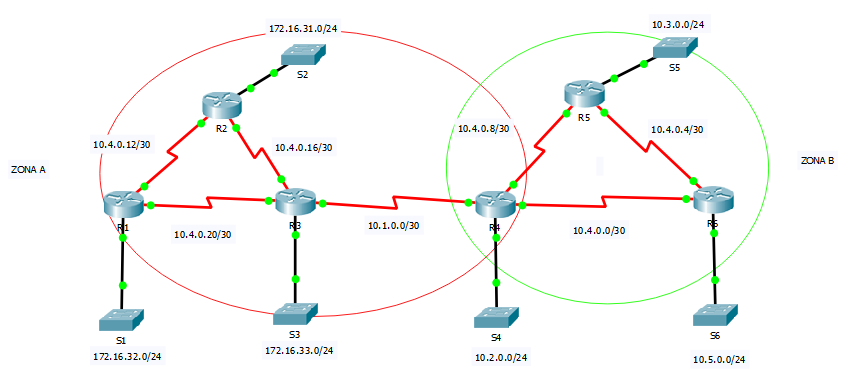
\includegraphics[scale=0.8]{img_ex2p.PNG}
\end{figure}

\section{Actividades a desarrollar (valor del examen: 15pts.)}
\subsection{Exploración de la topología}
Familiarícese con la topología. Tenga a mano los comandos de verificación de direccionamiento IP, enrutamiento dinámico y de configuración en ejecución.
 Utilice los comandos de verificación y responda las siguientes preguntas:
\begin{enumerate}[label=\Alph*]
\item ¿Cuáles Routers ejecutan EIGRP y con qué AS?
\item ¿Cuáles Routers ejecutan OSPF y con qué ID de proceso?
\end{enumerate}
Estas respuestas pueden guiarle para la siguiente parte del examen. Anótelas en una hoja y continúe con el desarrollo del examen. NOTA: para la configuración de EIGRP se ha utilizado la dirección de red y la wildcard.

\subsection{Configuraciones básicas}
\begin{enumerate}[label=\Alph*]
\item Añada un host a cada red. Configure el direccionamiento y verifique la conectividad entre LAN. ¿Hay conectividad total exitosa?
\end{enumerate}
\textit{\textbf{Si los mensajes en consola le dificultan la escritura de comandos, recuerde que configurar logging synchronous le ayuda evitar que los mensajes en consola interfieran con la escritura de comandos}} 

\subsection{Resolución de problemas}
\subsubsection{Respecto a \textbf{EIGRP} (5\%)}
\begin{enumerate}
\item Verifique si hay conectividad entre las redes locales de los routers que ejecutan EIGRP.
\item Analice cuáles serían los posibles problemas que presenta la zona EIGRP.
\item Haga los cambios necesarios en las configuraciones para que las LAN de la zona EIGRP tengan conectividad total.
\item Liste los problemas encontrados y la solución dada.
\end{enumerate}

\subsubsection{Respecto a \textbf{OSPF} (5\%)}
\begin{enumerate}
\item Verifique si hay conectividad entre las redes locales de los routers que ejecutan OSPF.
\item Analice cuáles serían los posibles problemas que presenta la zona OSPF.
\item Haga los cambios necesarios en las configuraciones para que las LAN de la zona OSPF tengan conectividad total.
\item Liste los problemas encontrados y la solución dada.
\end{enumerate}

\subsubsection{Configuración de redistribución de rutas (3\%)}
\begin{enumerate}
\item ¿En qué router se debe realizar la redistribución de rutas?
\item Redistribuya las rutas de EIGRP en el proceso OSPF
\item Redistribuya las rutas de OSPF en el proceso EIGRP (utilice la métrica que aparece en el guión de la práctica de redistribución de protocolos).
\item Verifique si hay conectividad total en la topología
\end{enumerate}

\textit{\textbf{Asegúrese de guardar las configuraciones en cada router, y guardar el archivo de packet tracer.}}

\subsection{Preguntas adicionales (2\%)}
\begin{enumerate}
\item ¿Cuál es la utilidad de desactivar el resumen automático de rutas al configurar EIGRP?
\item Referente a la topología: elimine el enlace serial entre R4 y R5. Espere unos segundos. ¿Tiene R1 una ruta para alcanzar los host de la red 10.3.0.0/24?
En caso de tenerla, ¿Cuál es su métrica? ¿Cuál es la distancia administrativa con la que fue marcada la ruta?
\end{enumerate}

\vfill
10 de agosto de 2018\\
José Mario López\\
\textit{Profesor de la asignatura}
\end{document}